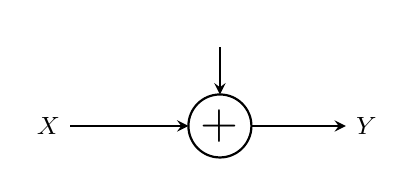
\begin{tikzpicture}
\shorthandoff{>}
%
%
% entrada
\draw[>=stealth,->,thick] (0,0) node[left]{\small $X$} --(1.5,0);
%
% adicion del ruido
\draw[thick] (1.9,0) circle (.4);
\draw[>=stealth,->,thick] (1.9,1) node[above]{\small $\N$} --(1.9,.4);
\node[align=center,scale=1.5] at (1.9,0){\large +};
%
% salida
\draw[>=stealth,->,thick] (2.3,0)--(3.5,0) node[right]{\small $Y$};
\end{tikzpicture}
